\documentclass[12pt,a4paper]{article}
\usepackage[margin=25mm]{geometry}
\usepackage[T1]{fontenc}
\usepackage{lmodern}
\usepackage{amsmath,amssymb,booktabs,tabularx,array}
\usepackage{setspace}
\usepackage{tikz}
\usetikzlibrary{arrows.meta,positioning,calc}
\usepackage{caption}
\usepackage[hidelinks]{hyperref}
\usepackage{microtype}
\onehalfspacing
\setlength{\parindent}{0pt}
\setlength{\parskip}{6pt}
\setlength{\emergencystretch}{2em}
\captionsetup{font=normalsize,labelfont=bf}
\newcolumntype{Y}{>{\raggedright\arraybackslash}X}
\newcolumntype{P}[1]{>{\raggedright\arraybackslash}p{#1}}
\title{Selective IMU Corrections and Cross-Question Consistency for Infrared Video Question Answering}
\author{Hanif Noer Rofiq\\Team Saw It\\\texttt{hanif.rofiq94@gmail.com}}
\date{CUHK-X Challenge 2026\quad Large Model Track\\28 September 2026}
\begin{document}
\maketitle
\begin{abstract}
Infrared video provides evidence about human activity, but some questions remain difficult to resolve from visible motion alone. This report describes the Saw It submission to the CUHK-X Large Model Track. The system combines Gemini video question answering with a Random Forest trained on wearable inertial measurements and a fixed rule that connects answers about the same clip. The classifier only replaces emotion answers when sufficient sensor data are available and its blended option scores meet a margin threshold. The consistency rule adds actions supported by exact text matches to a predicted combination answer. On a subject-held-out development set of 972 questions, the complete pipeline answered 768 correctly (79.01\%), compared with 743 (76.44\%) for the infrared baseline. Emotion corrections contributed a net gain of 20 answers and consistency contributed five. The selected submission received participant-confirmed public and private leaderboard scores of 0.78654 and 0.81176, respectively. The development set was inspected during method development, and fresh end-to-end API reproduction remains unverified. The result supports selective use of complementary information in this setting, without establishing general improvement across subjects, environments or API versions.
\end{abstract}

\section{Task and approach}
CUHK-X provides benchmarks for human activity recognition, understanding and reasoning across multiple sensor modalities~\cite{cuhkx}. Our entry addresses the Large Model Track's question-answering task using infrared (IR) video and inertial measurement unit (IMU) signals. Questions require a single choice, a set of actions, an ordered sequence, a combination of actions, an emotion description or an object interaction. The answer letters are specific to each question, so predictions must be mapped to the supplied options.

We used a hosted video-language model for the general question-answering stage. Emotion remained a substantial source of error, motivating a separate classifier for that category. A rule across questions then reused information already produced for the same clip. These components act on predictions rather than on a shared learned multimodal representation. The selected method uses no RGB, depth, thermal, radar or skeleton input. A later skeleton experiment did not improve the selected pipeline.

The following sections describe the submitted method, matched local comparisons and the artifacts available for reproduction. We distinguish development accuracy from the public and private leaderboard results and discuss the remaining limitations of the recovered package.

\section{Data and development protocol}
The official training QA file contains 4,087 questions. We held out subjects user4, user9, user19 and user24, giving 972 validation questions and 3,115 fitting questions. Every question and modality associated with a subject stays in the same partition. Subject identities, directory names and trial identifiers are routing metadata, not classifier features or text included in the video prompt.

Emotion accounts for 809 training questions, of which 620 belong to fitting subjects and 189 to held-out subjects. Usable IMU was available for 600 fitting and 187 validation emotion records. The local classifier and option prior were fitted using only usable records from fitting subjects. Four-fold subject-grouped inner validation selected the minimum leaf size from \{2,6\} and the prior weight from \{0,0.25,0.5\}; the chosen values were 6 and 0.5. The override margin was fixed at 0.10. Once the pipeline was selected, the classifier and prior were refitted on all 787 usable official training emotion records.

The split prevents direct subject overlap during development, but it was not an untouched final test. An initial 123-question pilot and previously inspected emotion validation results informed development before evaluation was extended to the full holdout. The final comparisons are descriptive development results.

No additional labelled external dataset or synthetic training set was used by the selected classifier. Gemini's pretraining data are not controlled by the team. Test labels, sample-submission predictions and manually assigned test answers were not used for fitting or model selection.

\begin{table}[htbp]
\centering
\caption{Sources used by the selected system. API pretraining knowledge is distinguished from labelled data used by our local classifier.}
\begin{tabularx}{\linewidth}{@{}P{0.25\linewidth}YP{0.18\linewidth}@{}}
\toprule Source & Role & Stage \\
\midrule
Official training QA & Emotion targets, option counts, grouped model selection and held-out evaluation & Development, training \\
Official training IMU & Motion features for the emotion classifier & Training \\
Official IR and QA & Video evidence, questions and answer options for validation and test clips & Development, inference \\
Official test IMU & Emotion features and signal availability & Inference \\
Gemini service & External pretrained knowledge accessed through a hosted model & Inference \\
\bottomrule
\end{tabularx}
\end{table}

\section{Method}
For question $i$, let $\mathcal{L}_i$ be its nonempty option letters, $t_{i\ell}$ the text of option $\ell$, and $g_i$ the legal answer returned by Gemini. The system first obtains all $g_i$ for a clip, then applies the consistency rule, and finally applies the IMU override to eligible emotion questions. These last two operations affect different categories. Figure~\ref{fig:framework} separates inference from the parameters learned using labelled training data.

% FRAMEWORK_BEGIN
\begin{figure}[htbp]
\centering
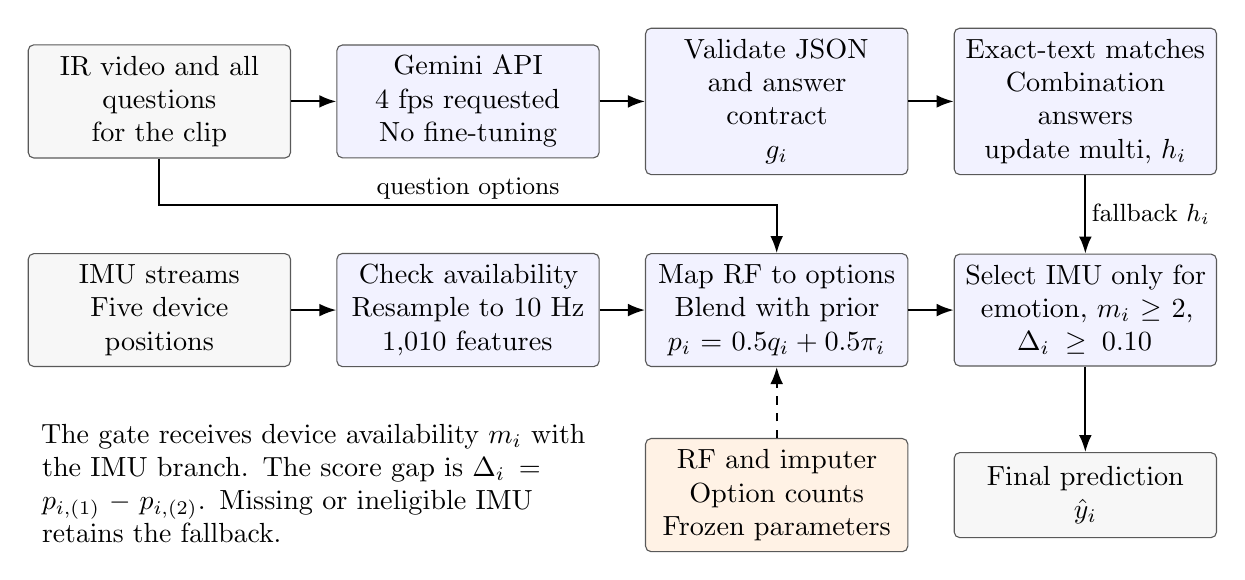
\begin{tikzpicture}[x=0.98cm,y=1cm,>=Latex,
 box/.style={draw=black!65,rounded corners=2pt,align=center,text width=3.05cm,minimum height=1.08cm,font=\fontsize{10}{12}\selectfont,inner sep=4pt},
 input/.style={box,fill=black!3},
 fixed/.style={box,fill=blue!5},
 learned/.style={box,fill=orange!10},
 arr/.style={->,line width=.7pt},
 lbl/.style={font=\fontsize{9}{11}\selectfont,fill=white,inner sep=2pt}]
\node[input] (ir) at (0,0) {IR video and all\\questions for the clip};
\node[fixed] (api) at (4,0) {Gemini API\\4 fps requested\\No fine-tuning};
\node[fixed] (parse) at (8,0) {Validate JSON\\and answer contract\\$g_i$};
\node[fixed] (cons) at (12,0) {Exact-text matches\\Combination answers\\update multi, $h_i$};
\draw[arr] (ir)--(api);
\draw[arr] (api)--(parse);
\draw[arr] (parse)--(cons);
\node[input] (imu) at (0,-2.65) {IMU streams\\Five device positions};
\node[fixed] (feat) at (4,-2.65) {Check availability\\Resample to 10 Hz\\1,010 features};
\node[fixed] (score) at (8,-2.65) {Map RF to options\\Blend with prior\\$p_i=0.5q_i+0.5\pi_i$};
\node[fixed] (select) at (12,-2.65) {Select IMU only for\\emotion, $m_i\geq2$,\\$\Delta_i\geq0.10$};
\draw[arr] (imu)--(feat);
\draw[arr] (feat)--(score);
\draw[arr] (score)--(select);
\draw[arr] (cons)--node[lbl,right]{fallback $h_i$}(select);
\draw[arr] (ir.south) -- (0,-1.32) -- node[lbl,above]{question options} (8,-1.32) -- (score.north);
\node[learned] (artifacts) at (8,-5.0) {RF and imputer\\Option counts\\Frozen parameters};
\draw[arr,dashed] (artifacts)--(score);
\node[input] (final) at (12,-5.0) {Final prediction\\$\hat y_i$};
\draw[arr] (select)--(final);
\node[align=left,font=\fontsize{10}{12}\selectfont,text width=6.9cm] at (2,-4.85)
{The gate receives device availability $m_i$ with the IMU branch. The score gap is $\Delta_i=p_{i,(1)}-p_{i,(2)}$. Missing or ineligible IMU retains the fallback.};
\end{tikzpicture}
\caption{Inference in the selected system. Solid arrows carry inputs or predictions; the dashed arrow supplies fixed parameters learned from official training records. The fallback $h_i$ is the video answer after consistency processing. Labelled training examples do not enter inference. The score mixture combines RF and prior probabilities, not Gemini probabilities.}
\label{fig:framework}
\end{figure}
% FRAMEWORK_END

\subsection{Infrared video question answering}
The recovered configuration identifies the service as \texttt{gemini-3.8-flash}. We upload the original IR MP4 and send all questions for that clip in one request, including category, question text and nonempty or blank A--D option fields. The prompt directs the model to use visible evidence, treat options as candidates and preserve each question's letter mapping. It requests timestamped observations and one answer for every question identifier. These observations are output text, not an independently supervised detector.

The request sets video sampling metadata to 4 fps, thinking level to \texttt{low}, an output budget of 8,192 tokens and a JSON schema. The API supports video input and configurable video processing~\cite{gemini}; 4 fps is a requested sampling rate, not a locally measured count of decoded frames. The client does not specify a spatial resizing rule, temperature or generation seed. We do not fine-tune the hosted model or supply labelled few-shot examples.

The parser checks coverage, unique identifiers and legal option letters. A multiple-answer prediction is treated as a set, while a sequence must contain every available letter exactly once in its predicted order. Invalid outputs can receive format feedback and another request using the video, without supplying correct labels. The original test workflow used asynchronous Batch inference; this is a scheduling choice, not a separate learned component.

\subsection{IMU representation and classifier}
The IMU branch reads the published upper- and lower-body CSV streams. It uses chest, left/right arm and left/right leg devices, represented by WTC, WTLA, WTRA, WTLL and WTRL. Each device provides three acceleration axes and three angular-velocity axes; acceleration and angular-velocity norms form two additional channels.

For each device, timestamps are sorted, duplicate timestamps averaged and valid channels linearly interpolated to a 10 Hz grid. A device is usable only with at least eight unique samples, duration between 0.7 and 300 seconds, and no timestamp gap longer than one second. Each channel contributes 25 features covering distribution summaries, root-mean-square differences, Hann-windowed spectral energy and frequency summaries, autocorrelation at three lags, and mean and standard deviation within each third of the recording. Device presence and duration contribute two further values. Five devices therefore produce $5(8\times25+2)=1{,}010$ features. Missing channel features are imputed using medians fitted on the relevant training subset.

A Random Forest~\cite{breiman} predicts the normalised text of the correct emotion description, not a globally fixed answer letter. It has 400 trees, minimum leaf size 6, \texttt{max\_features}=0.5 and random seed 20260913, with no class weighting. At inference, class probabilities are mapped to the descriptions offered in the current question and renormalised over its available options. Unseen descriptions receive zero RF mass. If every offered description receives zero mass, the implementation falls back to the option prior described below.

\subsection{Option prior and selective replacement}
For normalised description $t$, let $C(t)$ count its occurrences as the correct training option and $O(t)$ count how often it was offered. Counts use the same usable training records as the classifier. The smoothed score and question-specific prior are
\begin{equation}
 s(t)=\frac{C(t)+2}{O(t)+8},\qquad
 \pi_{i\ell}=\frac{s(t_{i\ell})}{\sum_{k\in\mathcal{L}_i}s(t_{ik})}.
\end{equation}
Let $q_{i\ell}$ denote the RF probability after mapping and renormalisation. The score used for prediction is
\begin{equation}
 p_{i\ell}=0.5q_{i\ell}+0.5\pi_{i\ell},\qquad
 r_i=\operatorname*{arg\,max}_{\ell\in\mathcal{L}_i}p_{i\ell}.
\end{equation}
The gap between the largest and second-largest scores is $\Delta_i=p_{i,(1)}-p_{i,(2)}$. If $m_i$ is the number of usable devices, the final answer is
\begin{equation}
 \hat y_i=\begin{cases}
 r_i,&\text{emotion question, }m_i\geq2\text{ and }\Delta_i\geq0.10,\\
 h_i,&\text{otherwise},
 \end{cases}
\end{equation}
where $h_i$ is the video prediction after consistency processing. A margin above 0.10 is an operational selection rule, not calibrated evidence that an answer is correct. The method can replace correct video answers as well as fix errors.

\subsection{Cross-question consistency}
For a clip with exactly one combination question, the rule takes the text of its predicted option, splits it on commas, case-folds it and collapses whitespace. Let $S_c$ be the resulting set of action strings. For each multiple-answer question from that clip, let $G_i$ be the original set of Gemini letters. The updated set is
\begin{equation}
 H_i=G_i\cup\{\ell\in\mathcal{L}_i:\operatorname{norm}(t_{i\ell})\in S_c\}.
\end{equation}
The result is serialised alphabetically. The rule only adds exact matches; it neither removes unsupported actions nor resolves synonyms. If the clip does not have exactly one combination question, the rule makes no change. Other categories retain their video predictions at this stage. For example, a selected combination containing ``walk, sit'' can add the letter for ``sit'' to a multiple-answer response that already includes ``walk''. This is an illustrative operation, not a manually labelled test example.

\section{Results}
\subsection{Local comparisons}
Table~\ref{tab:ablation} compares the same 972 held-out development questions. Accuracy uses exact answers, except that multiple-answer questions compare sets; sequences retain order. The IR baseline answers 743 questions correctly. IMU replacement contributes a net gain of 20, and consistency contributes five. Their combined gain is 25 answers, or 2.57 percentage points. Because the two additions affect different categories, this additive gain does not demonstrate a learned interaction between modalities.

\begin{table}[htbp]
\centering
\caption{Matched local development results. Fixes and regressions are measured against the IR baseline.}
\label{tab:ablation}
\begin{tabular}{@{}lrrrr@{}}
\toprule Pipeline & Correct & Accuracy & Fixes & Regressions \\
\midrule
IR baseline & 743 & 76.44\% & -- & -- \\
IR + consistency & 748 & 76.95\% & 6 & 1 \\
IR + IMU replacement & 763 & 78.50\% & 42 & 22 \\
Complete pipeline & 768 & 79.01\% & 48 & 23 \\
\bottomrule
\end{tabular}
\end{table}

The regressions matter when interpreting the margin rule. It limits replacement but does not make it uniformly beneficial. Table~\ref{tab:category} shows where the net gains occur. Emotion improves from 52/189 to 72/189, yet still accounts for 117 of the final 204 errors. Sequence questions also remain difficult. Neither added component changes sequence predictions.

\begin{table}[htbp]
\centering
\caption{Category results on the local development set. Counts are correct answers over the category total.}
\label{tab:category}
\begin{tabular}{@{}lrrr@{}}
\toprule Category & IR baseline & Complete pipeline & Final accuracy \\
\midrule
Single & 285/297 & 285/297 & 95.96\% \\
Combination & 175/185 & 175/185 & 94.59\% \\
Multiple-answer & 152/189 & 157/189 & 83.07\% \\
Sequence & 53/78 & 53/78 & 67.95\% \\
Emotion & 52/189 & 72/189 & 38.10\% \\
Object interaction & 26/34 & 26/34 & 76.47\% \\
\bottomrule
\end{tabular}
\end{table}
Questions from the same clip share evidence and are correlated. We therefore report direct counts rather than interpreting a row-level significance test as independent clip-level evidence. The holdout was inspected during development, and the reported accuracy is not a claim about an untouched population of unseen subjects.

\subsection{Submission and unsuccessful extension}
The selected CSV contains 682 predictions. The final RF was fitted on all 787 usable training emotion records; 139 of 144 test emotion records had usable IMU, and 81 met the replacement conditions. Relative to the original IR submission, 55 emotion answers and nine multiple-answer responses changed. Eligible replacement does not necessarily change an answer when both branches already agree.

The selected submission received a public leaderboard score of 0.78654 (78.654\%) and a private leaderboard score of 0.81176 (81.176\%). These results were confirmed by the participant. They are separate from the 79.01\% local development accuracy: the three evaluations use different partitions, so differences between their scores do not establish a controlled distribution-shift effect.

A separate skeleton GCN trial evaluated graph/IMU mixtures using grouped inner validation. Its selected graph weight was zero, with 280/620 correct inner-validation answers. The resulting outer predictions remained unchanged at 768/972. This experiment is evidence against including that tested configuration, not evidence that skeleton information is generally unhelpful. No skeleton model enters the selected CSV pipeline.

\section{Efficiency and reproduction}
The trained local components run on CPU and require no local GPU, PyTorch or CUDA. The historical final CPU refit took 141.50 seconds; this measurement is not the duration of full video inference. Full fresh-inference wall time and peak host memory have not been measured for the reconstructed entry point. The final reconstructed RF artifact occupies 3,824,746 bytes. Hosted-model computation, upload time and API charges remain external costs; CPU-only local processing does not make the complete system offline or free.

The package provides \texttt{inference.sh}, which accepts a data directory and output CSV path. It expects official label-free testing QA, IR clips and available IMU records. Credentials are supplied separately through the environment. The Python environment is pinned to Python 3.13.9, NumPy 2.3.5, pandas 2.3.3, SciPy 1.16.3, scikit-learn 1.7.2 and joblib 1.5.2, with transitive dependencies specified in \texttt{requirements.txt}. Training code uses the official training inputs and fixed parameters.

There are material limits to the recovered artifacts. After local cleanup, the selected CSV was recovered byte-for-byte, verified by its original SHA-256. Component source and sensor features were recovered, while the RF checkpoint was newly fitted using the frozen parameters. Its predictions agree with the selected CSV on all 81 eligible emotion records. All 144 test IMU feature vectors match the recovered cache exactly. These checks support the reconstruction but do not establish equality with the deleted checkpoint bytes.

Original raw Gemini responses and a returned immutable service revision are unavailable. The configuration records the alias \texttt{gemini-3.8-flash}; it does not pin the provider's underlying snapshot. The reconstructed portable wrapper uses sequential requests, whereas the original test run used Batch scheduling. Five offline wrapper tests passed, but fresh live-API and Linux end-to-end execution remain unverified. The selected CSV is retained as an output record and is never used to answer new private inputs. We cannot claim exact reproduction of the full leaderboard result from these checks alone.

\section{Discussion and limitations}
The main design choice is selective use of a small sensor classifier where the video model struggled. Late replacement keeps the two components independently inspectable and allows an explicit fallback for missing signals. Its cost is dependence on a fixed score threshold and training option frequencies. Changes in emotion wording, motion style, device placement or label proportions may reduce the usefulness of the classifier or prior. The development comparisons do not isolate whether the IMU features, prior or their mixture explains each corrected answer.

Cross-question consistency reuses a predicted relationship without another API request. It is limited by the correctness of the combination answer and by literal text matching. A mistaken combination can propagate an additional error, as the observed regression demonstrates. This rule is a task-specific constraint and should not be described as general logical reasoning.

The method uses non-RGB signals but does not establish anonymisation or clinical emotion recognition. Its emotion outputs are selections among dataset descriptions. Their low held-out accuracy and sensitivity to context make broader claims about a person's psychological state inappropriate. Future work would need an independent subject evaluation, clip-level uncertainty analysis and controlled changes in sensor availability before claiming robustness. These are limitations of the present evidence, not completed experiments.

\section{Conclusion}
The selected Saw It system combines infrared video-language inference, a fixed IMU-based emotion replacement rule and exact-text consistency across questions. On the inspected subject-held-out development set, the additions increase accuracy from 76.44\% to 79.01\%, while also introducing some regressions. The result motivates testing targeted sensor corrections and task-specific answer relationships under independent evaluation. The selected output file is preserved, but missing original API responses and an unpinned service snapshot remain obstacles to exact end-to-end reproduction.

\begin{thebibliography}{9}
\bibitem{cuhkx} Siyang Jiang, Mu Yuan, Xiang Ji, Bufang Yang, Zeyu Liu, Lilin Xu, Yang Li, Yuting He, Liran Dong, Wenrui Lu, Zhenyu Yan, Xiaofan Jiang, Wei Gao, Hongkai Chen, and Guoliang Xing. 2026. A Large-Scale Multimodal Dataset and Benchmarks for Human Activity Scene Understanding and Reasoning. In \emph{Proceedings of MobiSys '26}, 352--370. \url{https://doi.org/10.1145/3745756.3809209}.
\bibitem{breiman} Leo Breiman. 2001. Random Forests. \emph{Machine Learning} 45, 5--32. \url{https://doi.org/10.1023/A:1010933404324}.
\bibitem{gemini} Google. Gemini API video understanding documentation. Accessed 28 September 2026. \url{https://ai.google.dev/gemini-api/docs/video-understanding}.
\end{thebibliography}
\end{document}
